% Copyright (C) 2022-2023 Florin-Ioan Subțirică


\documentclass{article}

\usepackage{float}
\usepackage{tabularx}
\usepackage{siunitx}
\usepackage[a4paper, total={6in, 8in}]{geometry}
\usepackage[utf8]{inputenc}
\usepackage[english, romanian]{babel}
\usepackage[hidelinks]{hyperref}
\usepackage{indentfirst}
\usepackage[siunitx, RPvoltages]{circuitikz}
\usepackage{fancyhdr}
\usepackage{xspace}
\usepackage{amssymb}
\usepackage{layout}
\usepackage{lastpage}
\usepackage{titling}
\usepackage{leftidx}
\usepackage{array}
\usepackage{enumitem}
\usepackage{titletoc,tocloft}
\usepackage{xcolor}
\usepackage{amsmath}
\usepackage{nicefrac}
\usepackage{mathtools}
\usepackage{graphicx}
\graphicspath{ {./} }


% Configuring the \latex command with sane defaults
\newcommand{\latex}{\LaTeX\xspace}

% Configuring the margins and layout
\oddsidemargin  = 13pt
\headheight     = 12pt
\textheight     = 674pt
\marginparsep   = 10pt
\footskip       = 30pt
\hoffset        = 0pt
\paperwidth     = 597pt
\topmargin      = -23pt
\headsep        = 25pt
\textwidth      = 426pt
\marginparwidth = 50pt
\marginparpush  = 5pt
\voffset        = 0pt
\paperheight    = 845pt

% Removing default header & footer configuration
\fancyhf{}

% Configuring the header
\pagestyle{fancy}
\lhead[Fizică]{Fizică}
\rhead[Florin-Ioan Subțirică]{Florin-Ioan Subțirică}

% Configuring the footer
\fancyhf[FR]{Pagina \thepage\ din \pageref{LastPage}}

% Setting up links inside content table
\hypersetup {
    citecolor = black,
    filecolor = black,
    linkcolor = black,
    urlcolor  = black,
    colorlinks,
}

% Configuring the titlepage
\title          {Experiența Debye-Scherrer de difracție a electronilor pe o rețea policristalină}
\author         {Florin-Ioan Subțirică \\ Seria CD, Grupa 322}
\date           {24.10.2022}
\predate{\centering}

\postdate{\vfill\emph{Facultatea de Automatică și Calculatoare}\hspace{2cm} \\
                \emph{Universitatea Politehnica București}     \hspace{2cm} \\
          \hfill\emph{2022 - 2023}\hfill}

% Configuring the table of contents
\setlength{\cftsubsecindent}{1cm}
\setlength{\cftsubsubsecindent}{2cm}
\dottedcontents{section}[1.5em]{}{1.3em}{.6em}



%%%%%%%%%%%%%%%%%%%%%%%%%%%%%%%%%%%%%%%%%%%%%%%%%%%%%%%%%%%%%%%%%%%%%%%%%%%%%%%


\begin{document}

% Project title
\maketitle
\thispagestyle{empty} % Remove page number
\pagebreak

% Table of contents
\tableofcontents
\thispagestyle{empty}
\pagebreak

% Introduction
\section        {Scopul lucrării}

\begin{itemize}
    \item \makebox[6mm]{} Determinarea lungimii de undă asociată electronilor
    \item \makebox[6mm]{} Verificarea ecuației de Broglie
    \item \makebox[6mm]{} Determinarea constantelor de rețea a grafitului
\end{itemize}    

\section        {Teorie}

\makebox[1cm]{} În anul 1924 Louis de Broglie a sugerat că în afara proprietăţilor specifice de
particule, acestea pot avea şi caracter ondulator şi a presupus că lungimea de undă a undei
asociate unei particule libere este dată de relaţia: 

\begin{equation}
    \lambda = \frac{h}{p}
\end{equation}

unde: \newline

\makebox[1cm]{} p - impulsul particulei \newline
\makebox[1.53cm]{} h - constanta lui Planck \newline

\makebox[1cm]{} Această ipoteză, confirmată de experienţele de difracţie de electroni pe o reţea
cristalină de nichel făcute de Clinton Davisson şi Lester Germer în anul 1927, a fost extinsă
de la particulele libere la orice tip de particule. \newline
\makebox[1.5cm]{} În experimentul de faţă este demonstrat caracterul ondulator al electronilor printr-o
experienţă de difracţie de electroni pe o reţea policristalină de grafit, experiment cunoscut
sub numele de difractie Debye-Scherrer. \newline
\makebox[1.53cm]{} Un fascicol de electroni monocromatici emişi de catodul unui tub electronic sunt
focalizaţi de un sistem de lentile electromagnetice şi cad pe o folie policristalină de grafit.
Atomii grafitului sunt aranjaţi într-o reţea cristalină care acţionează ca o reţea de difracţie
pentru electroni, pe un ecran fluorescent apărând figura de difracţie sub forma a două inele
concentrice (Figura 1) corespunzătoare celor două constante de reţea d1 şi d2 (Figura 3).
Diametrul inelelor concentrice se modifică în funcţie de lungimea de undă a electronilor şi,
deci, in funcţie de tensiunea de accelerare, conform consideraţiilor de mai jos. \newline

Energia unui electron accelerat de o diferenţă de potenţial (tensiune) U este: 

\begin{equation}
    eU = \frac{p^2}{2m}
\end{equation}

unde: \newline

\makebox[1cm]{} U - tensiunea de accelerare; \newline
\makebox[1.53cm]{} e - sarcina electronului; \newline
\makebox[1.53cm]{} p - impulsul electronului. \newline

\begin{figure}[H]
    \centerline{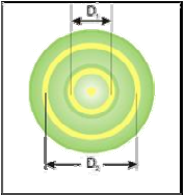
\includegraphics{fig1.png}}
    \caption{Reprezentarea schematică a inelelor de difracţie. Cele două inele cu diametrele
    \centerline{${D}{_1}$ și ${D}{_2}$ corespund constantelor de rețea ${d}{_1}$ și ${d}{_2}$ (conform Figura 3)}}
    \label{Fig}
\end{figure}

Separând impulsul p din ecuația (2) se obține $p = \sqrt{2meU}$, iar din ecuația (1) rezultă:
\begin{equation}
    \lambda = \frac{h}{\sqrt{2meU}}
\end{equation}

expresie care arată că lungimea de undă $\lambda$ depinde de tensiunea de accelerare U. \newline

\makebox[1cm]{} În anul 1913 sir H. W. Bragg şi fiul său W. L. Bragg au înteles că aranjarea
periodică a atomilor în reţeaua cristalină a unui monocristal este formată din plane
cristaline paralele. Dacă pe un set de astfel de plane cristaline cade un fascicol
monocromatic de raze X sau electroni monoenergetici care se presupune că au caracter
ondulatoriu, fiecare element al planului cristalin acţionează ca un centru de împrăştiere
generând o undă sferică elementară reflectată, suprapunerea acestor unde sferice
elementare generând un front de undă reflectat. Conform legilor reflexiei, lungimea de
undă a undei reflectate este aceeaşi cu a undei incidente si unghiul de reflexiei este egal cu
unghiul de incidenţă. Din suprapunerea undelor reflectate pe plane succesive se obţin
maxime de interferenţă (interferenţă constructivă) dacă diferenţa de drum $\Delta = {\Delta}{_1} + {\Delta}{_2} = 2d\sin{\theta}$ (Figura 2) este un multiplu întreg de lungimi de undă: 

\begin{equation}
    2d\sin{\theta} = n\lambda, n = 1,2,3,...
\end{equation}

unde: \newline

\makebox[1cm]{} d - distanţa dintre două plane succesive; \newline
\makebox[1.53cm]{} $\theta$ - unghiul de incidență măsurat față de plan. \newline

\makebox[1cm]{} Condiţia (4) este cunoscută ca relaţia Bragg.  \newline

\begin{figure}[H]
    \centerline{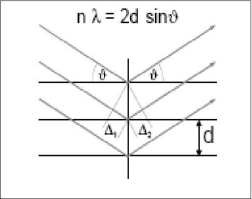
\includegraphics[scale = 0.6]{fig2.png}}
    \caption{Reprezentarea schematică a condiției de difracție Bragg}
    \label{Fig}
\end{figure}

\begin{figure}[H]
    \centerline{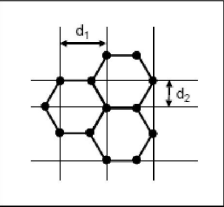
\includegraphics[scale = 0.6]{fig3.png}}
    \caption{Constantele de rețea în grafit: ${d}{_1} = 2,13 \cdot 10^{-10}$ m; ${d}{_2} = 1,23 \cdot 10^{-10}$ m}
    \label{Fig}
\end{figure}

\bigskip

\makebox[1cm]{} În experimentul din această lucrare se foloseşte un material policristalin care este
format dintr-un număr foarte mare de monocristale (cristalite) aranjate neregulat in spaţiu.
Vor exista totdeauna câteva monocristale a căror orientare satisface condiţia Bragg pentru
o lungime de undă şi direcţie a fascicolului incident date. Totalitatea reflexiilor produse de
aceste cristalite se află într-un con a cărui axă este dată de direcţia fascicolului incident,
astfel că pe ecranul aflat perpendicular pe această axa vor apărea cercuri concentrice.
Planele cristaline importante pentru figura de difracţie din acest experiment sunt, conform
Figura 3. \newline 

\begin{figure}[H]
    \centerline{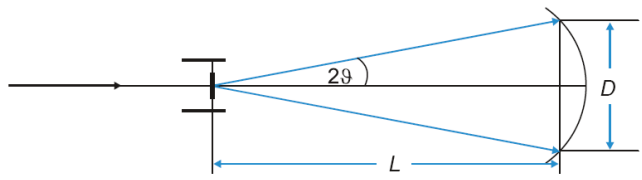
\includegraphics[scale = 0.6]{fig4.png}}
    \caption{Reprezentarea schematică a difracţiei Debye-Scherrer}
    \centerline{L=13,5cm (distanţa dintre stratul de grafit şi ecran)}
    \centerline{D este diametrul inelului de difracţie observat pe ecran}
    \label{Fig}
\end{figure}

\makebox[1cm]{} Din Figura 4 se obține relația:

\begin{equation}
    \tan{2\Theta} = \frac{D}{2L}
\end{equation}

unde: \newline

\makebox[1cm]{} D - diametrul unui inel; \newline
\makebox[1.53cm]{} L - distanţa de la probă la ecran. \newline

\makebox[1cm]{} Pentru unghiuri $\Theta$ mici:

\begin{equation}
    \tan{2\Theta} \approx \sin{2\Theta} \approx 2\sin{\Theta}
\end{equation}

\makebox[1cm]{} Substituind (6) în (4) se obţine, pentru primul ordin de difracţie n = 1, expresia
pentru lungimea de undă asociată electronilor: 

\begin{equation}
    \lambda = d\frac{D}{2L}
\end{equation}

\makebox[1cm]{} Ţinând cont de ecuaţia (3) se obţine pentru diametrul inelelor de difracţie: 

\begin{equation}
    D = k(d)\frac{1}{\sqrt{U}}
\end{equation}

\makebox[1cm]{} unde

\begin{equation}
    k(d) = \frac{2hL}{d\sqrt{2me}}
\end{equation}

\makebox[1cm]{} este panta dreptei $D = D(\frac{1}{\sqrt{U}})$, pantă care depinde de constanta de rețea d.

\section        {Descrierea instalației experimentale}

\makebox[1cm]{} Tubul electronic (de fapt, un tub catodic) în care apare fenomenul este reprezentat
în Figura 5. Conexiunile dintre tub şi sursa de înaltă tensiune sunt reprezentate în Figura 6. 

\begin{figure}[H]
    \centerline{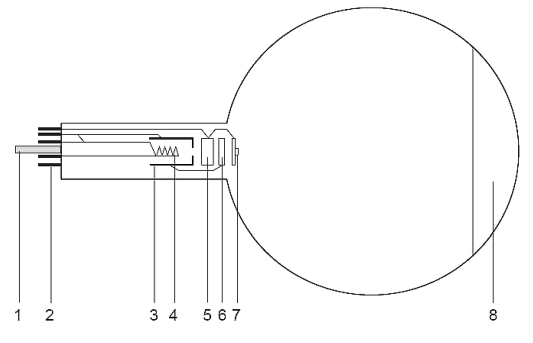
\includegraphics[scale = 0.6]{fig5.png}}
    \caption{}
    \label{Fig}
\end{figure}

unde \newline

\makebox[1cm]{} 1 - pin de ghidare cu cheiţă;  \newline
\makebox[1.53cm]{} 2 - pini de conexiune electrică;  \newline
\makebox[1.53cm]{} 3 - catod;  \newline
\makebox[1.53cm]{} 4 - filament de încălzire a catodului;  \newline
\makebox[1.53cm]{} 5 - anod;  \newline
\makebox[1.53cm]{} 6 - electrod de focalizare;  \newline
\makebox[1.53cm]{} 7 - strat subţire de grafit policristalin;  \newline
\makebox[1.53cm]{} 8 - ecran florescent (aici apar inelele de difracţie).  \newline

\begin{figure}[H]
    \centerline{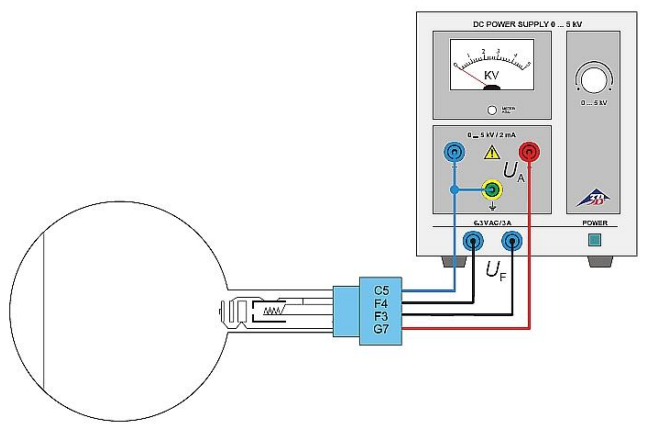
\includegraphics[scale = 0.6]{fig6.png}}
    \caption{Schema conexiunilor (a se respecta culorile cablurilor, în caz contrar}
    \centerline{instalaţia putând fi distrusă)}
    \label{Fig}
\end{figure}

\makebox[1cm]{} Sursa de înaltă tensiune este prezentă în două versiuni: una veche, mai mare ca
gabarit, cu afisaj analogic şi una nouă, mai mică, cu afişaj digital pentru tensiunea furnizată
(0-5 kV). Ambele tipuri de surse au aceleaşi borne de conexiuni, astfel că Fig. 6 este bună
indiferent de sursă. 

\section        {Modul de lucru}

\begin{itemize}
    \item \makebox[6mm]{} Am aplicat o tensiune de accelerare $U \leq 5k\si{\volt}$, putând astfel observa figura de difracție
    \item \makebox[6mm]{} Am variat tensiunea între 3k\si{\volt} și 5k\si{\volt}, treptat câte 0,5k\si{\volt}, astfel măsurând diametrele ${D}{_1}$ și ${D}{_2}$ ale inelelor de difracție observate pe ecran
    \item \makebox[6mm]{} Pentru a avea o acuratețe cât mai bună, fiecare membru al echipei a măsurat de 3 ori fiecare diametru, după care am făcut o medie per membru, iar mai apoi o medie totală. Rezultatele experimentale le-am trecut în Tabelul 1.
\end{itemize}

\begin{table}[H]
    \begin{tabular}{|c|c|c|c|c|c|c|c|c|}
    \hline
    {\color[HTML]{000000} U(kV)} & {\color[HTML]{000000} ${D}{_{1}{_I}}$(cm)} & {\color[HTML]{000000} ${D}{_{1}{_{II}}}$(cm)} & {\color[HTML]{000000} ${D}{_{1}{_{III}}}$(cm)} & {\color[HTML]{000000} ${D}{_{2}{_I}}$(cm)} & {\color[HTML]{000000} ${D}{_{2}{_{II}}}$(cm)} & {\color[HTML]{000000} ${D}{_{2}{_{III}}}$(cm)} & {\color[HTML]{000000} ${D}{_1}$(cm)} & {\color[HTML]{000000} ${D}{_2}$(cm)} \\ \hline
    {\color[HTML]{000000} 3}     & {\color[HTML]{000000} 2.9000}  & {\color[HTML]{000000} 2.9500}   & {\color[HTML]{000000} 3.0000}    & {\color[HTML]{000000} 5.0500}  & {\color[HTML]{000000} 5.0000}   & {\color[HTML]{000000} 5.0000}    & {\color[HTML]{000000} 2.9500} & {\color[HTML]{000000} 5.0167} \\ \hline
    {\color[HTML]{000000} 3.5}   & {\color[HTML]{000000} 2.6500}  & {\color[HTML]{000000} 2.7000}   & {\color[HTML]{000000} 2.7500}    & {\color[HTML]{000000} 4.5500}  & {\color[HTML]{000000} 4.6000}   & {\color[HTML]{000000} 4.6500}    & {\color[HTML]{000000} 2.7000} & {\color[HTML]{000000} 4.6000} \\ \hline
    {\color[HTML]{000000} 4}     & {\color[HTML]{000000} 2.5000}  & {\color[HTML]{000000} 2.5500}   & {\color[HTML]{000000} 2.5500}    & {\color[HTML]{000000} 4.2500}  & {\color[HTML]{000000} 4.3000}   & {\color[HTML]{000000} 4.3500}    & {\color[HTML]{000000} 2.5333} & {\color[HTML]{000000} 4.3000} \\ \hline
    {\color[HTML]{000000} 4.5}   & {\color[HTML]{000000} 2.3500}  & {\color[HTML]{000000} 2.3500}   & {\color[HTML]{000000} 2.4000}    & {\color[HTML]{000000} 4.0500}  & {\color[HTML]{000000} 4.0000}   & {\color[HTML]{000000} 4.1500}    & {\color[HTML]{000000} 2.3667} & {\color[HTML]{000000} 4.0667} \\ \hline
    {\color[HTML]{000000} 5}     & {\color[HTML]{000000} 2.2500}  & {\color[HTML]{000000} 2.2500}   & {\color[HTML]{000000} 2.3000}    & {\color[HTML]{000000} 3.8500}  & {\color[HTML]{000000} 3.8000}   & {\color[HTML]{000000} 3.8000}    & {\color[HTML]{000000} 2.2667} & {\color[HTML]{000000} 3.8167} \\ \hline
    \end{tabular}
    \end{table}

\section        {Prelucrarea rezultatelor experimentale}

\subsection{Determinarea lungimii de undă asociată electronilor}

\makebox[1cm]{} Primul pas a fost să calculăm valorile medii ale diametrelor inelelor de difracție.
După care, din valorile medii ale diametrelor inelelor de difracție ${D}{_1}$ și ${D}{_2}$ și valorile constantei de rețea ${d}{_1}$ și ${d}{_2}$
presupuse cunoscute (Figura 3), folosind ecuația (7) se poate obține lungimea de undă experimentală a electronilor.
${\lambda}{_{1}{_exp}}$ și ${\lambda}{_{2}{_exp}}$ (ambele scalate în pm) se calculează cu ajutorul lui ${D}{_1}$, ${d}{_1}$, și respectiv lui ${D}{_2}$, ${d}{_2}$.

\subsection{Verificarea relației de Broglie}

\makebox[1cm]{} Relația de Broglie (1) se verifică folosind ecuația (3) prin calcularea valorii teoretice a lungimii de
undă ${\lambda}{_t}$ (scalată tot în pm), unde:

\begin{equation*}
    e = 1.602 \cdot 10^{-19} \si{\coulomb}
\end{equation*}

\begin{equation*}
    m = 9.109 \cdot 10^{-31} \si{\kilogram}
\end{equation*}

\begin{equation*}
    h = 6.625 \cdot 10^{-34} \si{\joule\sec}
\end{equation*}

\makebox[1cm]{} Rezultatele sunt trecute în Tabelul 2, alături de datele experimentale (diametrele inelelor de difracţie). Se observă faptul că valorile lungimilor de undă de pe fiecare linie sunt apropiate.

\begin{table}[H]
    \begin{tabular}{|c|c|c|c|c|c|c|}
    \hline
    {\color[HTML]{000000} U(kV)} & {\color[HTML]{000000} \begin{tabular}[c]{@{}c@{}}$\frac{1}{\sqrt{U}}$\\ $(V^{-\frac{1}{2}})$\end{tabular}} & {\color[HTML]{000000} \begin{tabular}[c]{@{}c@{}}${D}{_1}$\\ (cm)\end{tabular}} & {\color[HTML]{000000} \begin{tabular}[c]{@{}c@{}}${D}{_2}$\\ (cm)\end{tabular}} & {\color[HTML]{000000} \begin{tabular}[c]{@{}c@{}}${\lambda}{_{1}{_{exp}}}$\\ (pm)\end{tabular}} & {\color[HTML]{000000} \begin{tabular}[c]{@{}c@{}}${\lambda}{_{2}{_{exp}}}$\\ (pm)\end{tabular}} & {\color[HTML]{000000} \begin{tabular}[c]{@{}c@{}}${\lambda}{_t}$\\ (pm)\end{tabular}} \\ \hline
    {\color[HTML]{000000} 3}     & {\color[HTML]{000000} 0.018257}                                                         & {\color[HTML]{000000} 2.9500}                                                   & {\color[HTML]{000000} 5.0167}                                                   & {\color[HTML]{000000} 23.272}                                                                   & {\color[HTML]{000000} 22.854}                                                                   & {\color[HTML]{000000} 22.389}                                                         \\ \hline
    {\color[HTML]{000000} 3,5}   & {\color[HTML]{000000} 0.016903}                                                         & {\color[HTML]{000000} 2.7000}                                                   & {\color[HTML]{000000} 4.6000}                                                   & {\color[HTML]{000000} 21.300}                                                                   & {\color[HTML]{000000} 20.956}                                                                   & {\color[HTML]{000000} 20.729}                                                         \\ \hline
    {\color[HTML]{000000} 4}     & {\color[HTML]{000000} 0.015811}                                                         & {\color[HTML]{000000} 2.5333}                                                   & {\color[HTML]{000000} 4.3000}                                                   & {\color[HTML]{000000} 19.985}                                                                   & {\color[HTML]{000000} 19.589}                                                                   & {\color[HTML]{000000} 19.390}                                                         \\ \hline
    {\color[HTML]{000000} 4.5}   & {\color[HTML]{000000} 0.014907}                                                         & {\color[HTML]{000000} 2.3667}                                                   & {\color[HTML]{000000} 4.0667}                                                   & {\color[HTML]{000000} 18.671}                                                                   & {\color[HTML]{000000} 18.526}                                                                   & {\color[HTML]{000000} 18.281}                                                         \\ \hline
    {\color[HTML]{000000} 5}     & {\color[HTML]{000000} 0.014142}                                                         & {\color[HTML]{000000} 2.2667}                                                   & {\color[HTML]{000000} 3.8167}                                                   & {\color[HTML]{000000} 17.882}                                                                   & {\color[HTML]{000000} 17.387}                                                                   & {\color[HTML]{000000} 17.343}                                                         \\ \hline
    \end{tabular}
    \end{table}

\subsection{Determinarea constantei de rețea a grafitului}

\makebox[1cm]{} Am reprezentat grafic ${D}{_1}$ și ${D}{_2}$ în funcție de $\frac{1}{\sqrt{U}}$.
Așa cum arată ecuația (8), rezultă două drepte (regresii lineare ale punctelor experimentale), pantele lor ${k}{_1}({d}{_1})$
și respectiv ${k}{_2}({d}{_2})$ satisfăcând ecuația (9). Folosind un script Python am generat graficul (Figura 7) ce pune în evidență atât punctele
reprezentate, cât și dreptele de regresie aferente. Același script calculează și panta fiecărei drepte.

\begin{figure}[H]
    \centerline{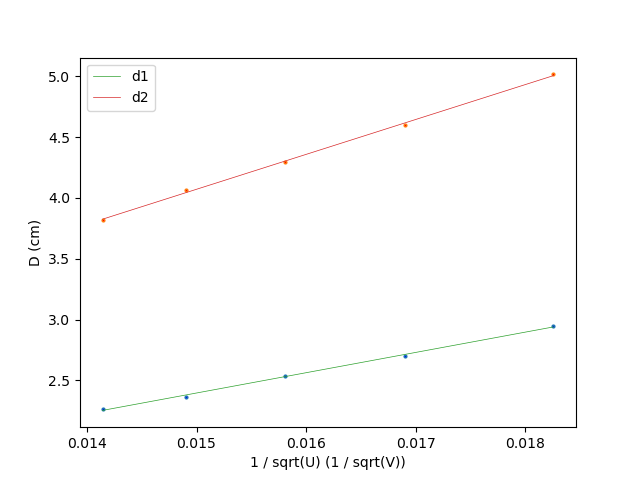
\includegraphics[scale = 0.5]{Plot.png}}
    \caption{Dreptele de regresie}
    \label{Fig}
\end{figure}

\makebox[1cm]{} Pantele dreptelor sunt:

\begin{equation*}
    {k}{_1}({d}{_1}) \approx 1.6690639046
\end{equation*}

\begin{equation*}
    {k}{_2}({d}{_2}) \approx 2.8703597613
\end{equation*}

\makebox[1cm]{} Folosind ecuația (9) obținem:

\begin{equation*}
    {d}{_1} \approx 1.9838 \cdot 10^{-10}
\end{equation*}

\begin{equation*}
    {d}{_2} \approx 1.1535 \cdot 10^{-10}
\end{equation*}

\makebox[1cm]{} , care sunt valori apropiate de cele evidențiate în Figura 3.

\section{Anexă}
\space\space\space\space \href{https://ctipub-my.sharepoint.com/:f:/g/personal/florin_subtirica_stud_acs_upb_ro/Eq0TbKFmnjhAoszjx_vnN18Bn3oi9FP3BmvfzAQFApd__Q?e=SbfAlY}{Referat} \newline

\begin{thebibliography}{10}

    $\href{http://www.physics.pub.ro/Referate/BN120/Experienta_DEBYE-SCHERRER_de_difractie_a_electronilor_pe_o_retea_policristalina_(2020).pdf}{Teorie}$

\end{thebibliography}
        
    \addcontentsline{toc}{section}{Bibliografie}

\end{document}

%%%%%%%%%%%%%%%%%%%%%%%%%%%%%%%%%%%%%%%%%%%%%%%%%%%%%%%%%%%%%%%%%%%%%%%%%%%%%%%
